\chapter{Planificación}
Para empezar a desarrollar la solución al problema, primero hay que establecer la metodología de su desarrollo y
control de calidad.\\

\section{Metodología utilizada}
Para el desarrollo del proyecto, tenía claro que quería utilizar una metodología basada en los principios del
manifiesto ágil\cite{agile}. Éstas se basan en la aportación frecuente de código que tenga valor para el usuario, lo
permite una rápida retroalimentación por parte de los usuarios y hace que el desarrollo sea muy flexible a posibles
cambios en alguna funcionalidad.\\

Las metodologías de desarrollo basadas en dichos principios más utilizadas son Kanban\cite{kanban} y Scrum\cite{scrum}.
Scrum se basa en ciclos cortos de trabajo en los que cada periodo determinado de tiempo \(lo más corto posible,
usualmente una o dos semanas\), el cliente recibe un avance en el código de acuerdo a una previa planificación de los
desarrolladores. Esta metodología es perfecta para empresas, ya que facilita las reuniones con los clientes al fijar la
duración de los ciclos y les permite saber de antemano en qué están trabajando los desarrolladores en cada ciclo,
sabiendo qué se van a encontrar en la siguiente versión del proyecto y permitiéndoles influir en la planificación de
los ciclos en base a las funcionalidades más prioritarias para ellos.\\

Aunque la metodología scrum resulta muy útil cuando hay un cliente al que satisfacer con tiempos de entrega y para
planificar de acuerdo a unas prioridades las tareas a realizar por un equipo de trabajo. En este proyecto en el que no
hay un cliente, por lo que es flexible en cuanto a tiempos de entrega, y solo hay un desarrollador, no le estaría
sacando el máximo partido a la metodología scrum.\\

Por tanto, para el desarrollo del proyecto, se optado por seguir la metodología Kanban. Que permite un seguimiento
visual del proyecto en el que se puede ver en todo momento qué tareas se deben hacer, cuáles están en desarrollo y
cuáles se han terminado ya. Apoyándonos en una tabla Kanban los usuarios pueden ver en todo momento el estado del
proyecto y las nuevas funcionalidades en las que se está trabajando. \\
% TODO: Introducir tabla cuando avances con las HU

\subsection{Seguimiento del desarrollo}
Para la transparencia y visualización del proyecto a lo largo de sus diferentes fases, debemos de poder acceder a
estados anteriores en su desarrollo. Para ello, utilizaremos Git, un sistema de control de versiones, en el que
fácilmente podemos ver versiones anteriores del proyecto e incluso volver a ellas revirtiendo algunos cambios,
aumentando la adaptabilidad del proyecto a cambios en los requerimientos de los usuarios.\\

Para alojar el código y registrar las tareas a realizar se ha optado por GitHub, ya que con una cuenta de estudiante
nos da acceso a la creación de tableros Kanban, como el mostrado anteriormente, para la organización de las tareas y a
la integración continua, de la que hablaremos más adelante, a través de las GitHub Actions.

De esta forma, los \textit{stakeholders}, o personas interesadas en el desarrollo del proyecto, podrán ver en todo
momento en qué fase del desarrollo se encuentra el mismo, y en qué estado está cada una de sus funcionalidades.\\

\subsection{Milestones}
Las milestones son los productos mínimamente viables del proyecto. Están formadas por documentos para organización del
trabajo que completan el PMV.\\

Éstos documentos son:
\begin{itemize}
    \item \href{https://github.com/Torchu/flixbuff/labels/user story}{\textbf{Historias de Usuario}}. Requerimientos
    propuestos por los usuarios de la aplicación, que definen una funcionalidad.
    \item \href{https://github.com/Torchu/flixbuff/labels/issue}{\textbf{Issues}}. Fallos o problemas en la aplicación
    que han de ser resueltos.
    \item \href{https://github.com/Torchu/flixbuff/labels/dev task}{\textbf{Tareas para el desarrollador}}. Pequeñas
    tareas que no representan una funcionalidad como tal.
\end{itemize}

Todas las tareas estarán asociadas a una issue diferente y tendrán una etiqueta acorde a su tipo y todo cambio en el
proyecto debe realizarse cumpliendo una tarea.
\begin{figure}[H]
	\centering	
	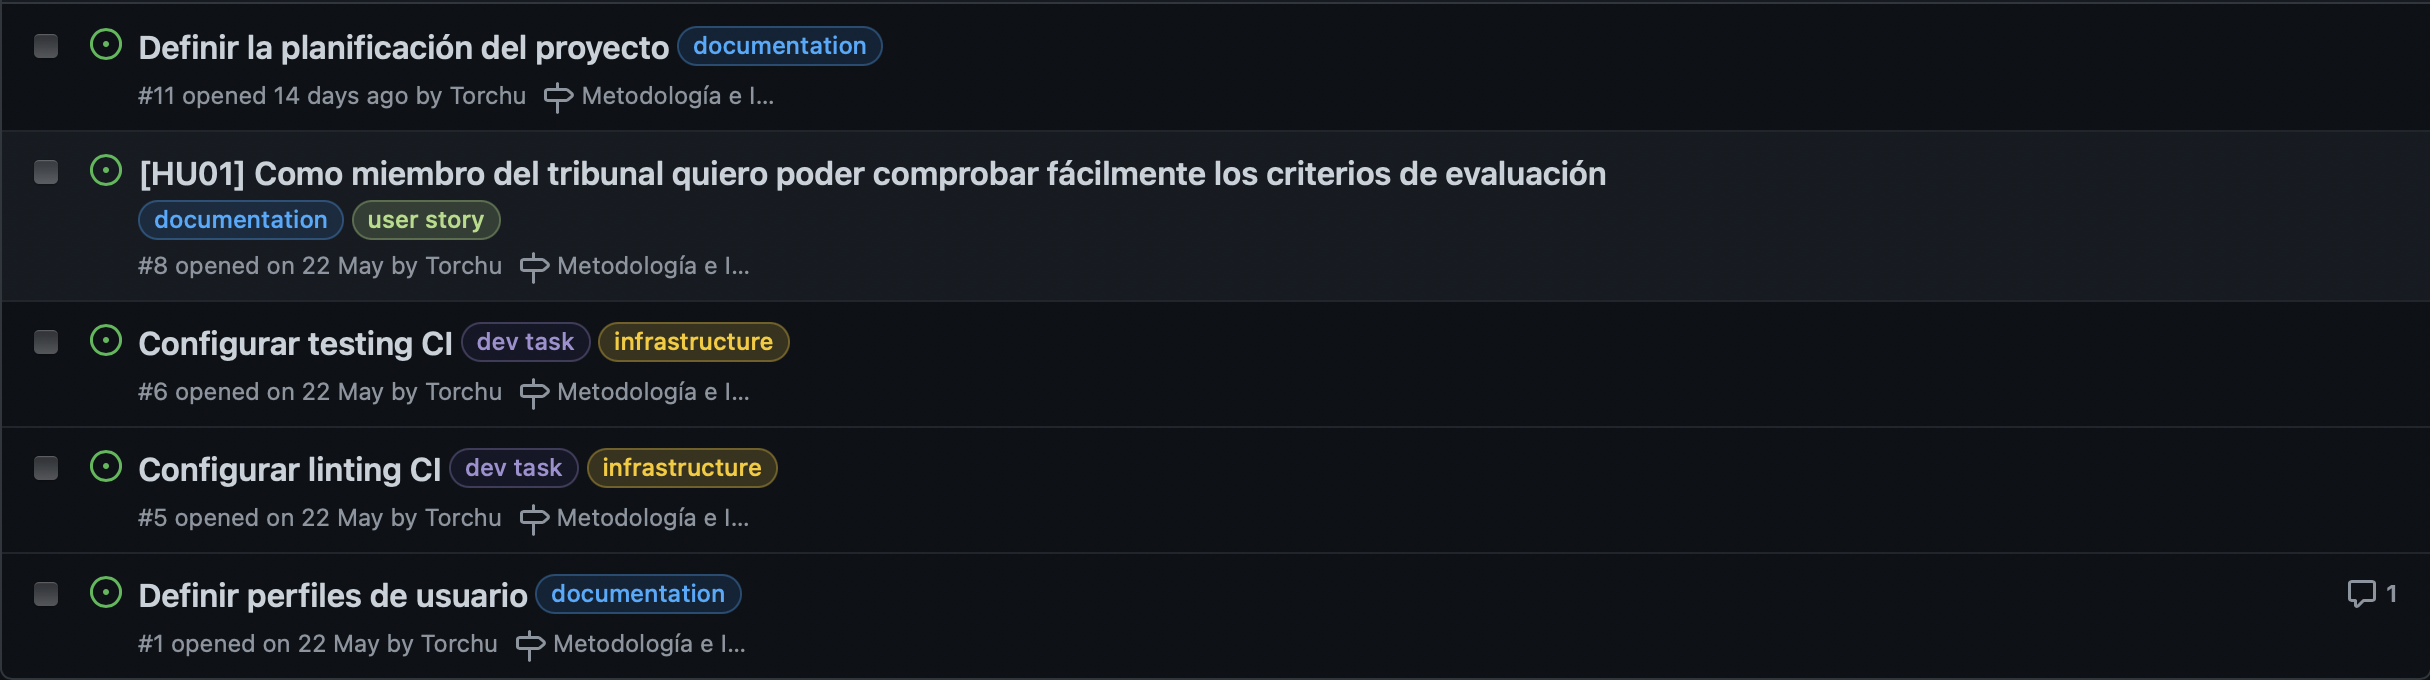
\includegraphics[scale=0.25]{img/issues.png}
	\caption{\href{https://github.com/Torchu/flixbuff/issues}{Issues} del proyecto}\label{fig:github_issues}
\end{figure}

Los milestones creados son visibles desde el repositorio de GitHub:
% TODO: Listarlos, poner links, etc.
% Son la infraestructura, el modelo de datos, el servicio de back y ambos front-end

\subsection{Historias de usuario}
Una historia de usuario es una funcionalidad que el usuario espera en la solución del problema. Es decir, un
requerimiento del usuario.\\

% TODO: Introducir imagen cuando avances con alguna HU

Como en este proyecto no tenemos unos usuarios que nos pidan los requisitos, se ha realizado un análisis de
\textit{Personas}\cite{personas}. Estas personas representan los perfiles de distintos usuarios de la aplicación y
serán ellos quienes nos ayuden con el disñeo del producto general, protagonizando las historias de usuario. Ver
\autoref{chap:personas}.\\

\section{Control de calidad}\label{sec:control_de_calidad}
Para asegurar la calidad del proyecto se ha seguido desde el comienzo del proyecto el desarrollo guiado por pruebas o
TDD\cite{TDD}.\\

Basándonos en esta metodología de desarrollo, trasladaremos los requisitos a una serie de pruebas dentro de nuestro
código, que se crearán antes del desarrollo de las funcionalidades. De esta forma, se convierten tanto en una
documentación fiable, que comprueba que el código desarrollado cumple los requisitos, como en una herramienta de
seguridad, que nos asegura que el código permanezca siempre correcto cada vez que se produzca algún cambio en el
mismo.\\
% TODO: Incluir imágenes de algún test

Además del desarrollo guiado por pruebas, se han configurado una serie de \textit{linters}. Unas herramientas que
comprueban que la sintáxis del código es correcta y cumplimenta la guía de estilo del lenguaje de programación en el
que está desarrollado, dando al desarrollador retroalimentación automática, reduciendo los costes de los posibles
cambios futuros, tal y como establece el dearrollo ágil.\\

Finalmente, se ha incluido un \textit{script} que comprueba la ortografía de toda la documentación del proyecto.
Sirviendo como un \textit{linter} para la documentación.\\

\subsection{Integración continua}

La integración continua es una metodología de trabajo que se basa en realizar integraciones frecuentes del código y
asegurarnos que superen los distintos controles de calidad, necesaria para respetar el noveno principio del manifiesto.
ágil:
\begin{quote}
    Continuous attention to technical excellence and good design enhances agility.
\end{quote}


Estos controles de calidad se comprueban mediante las \textit{pipelines}, o acciones que se ejecutan al subir código
al repositorio de GitHub. En nuestro caso incluiremos todo lo mencionado en el apartado
\hyperref[sec:control_de_calidad]{anterior}: pruebas de funcionalidad, \textit{linters} y revisión ortográfica.\\

Para este proyecto,se han configurado las \textit{pipelines} con la herramienta GitHub Actions. Se ha escogido esta
herramienta, ya que es propia de GitHub, la plataforma en la que se aloja el código del proyecto, por lo que no
necesitaremos configurar una herramienta externa. Además, es muy fácil de configurar. Simplemente incluyendo un fichero
yaml en el directorio \textit{.github/workflows/} la propia plataforma ya es capaz de reconocer y ejecutar las
\textit{pipelines} que se han configurado.\\

Se ha optado por una única herramienta para las \textit{pipelines}, ya que al tener solo una reduce el mantenimiento de
la infraestructura y aumenta la velocidad de los despliegues. Quizá en otros proyectos sea interesante mantener dos
herramientas, ya que si hay algún problema en una, no se detiene la integración de código. En este caso, al ser la
herramienta propia de la plataforma en la que se aloja el código, si se cae la plataforma, tampoco podríamos integrar
nuevo código al proyecto, por lo que no es necesaria una segunda herramienta.

% TODO: Incluir fotos aquí también cuando se hayan configurado el resto de GitHub Actions
